\documentclass[preprint,12pt,authoryear]{elsarticle}
\biboptions{authoryear,round,semicolon}
% \citet{smith2020}  % Smith (2020)
% \citep{smith2020}  % (Smith, 2020)



\usepackage[english]{babel}
\usepackage{amssymb,amsmath,amsfonts,amsthm}
\usepackage[most]{tcolorbox}
\newtheorem{lemma}{Lemma}
\usepackage{threeparttable}
\usepackage{xcolor}
\usepackage{longtable}
\usepackage{url}
\usepackage{multirow}
\usepackage{soul}
\usepackage{xcolor}
\usepackage{bbm}
\usepackage[most]{tcolorbox}
\usepackage{amsmath, amssymb}

\usepackage{soul}
\usepackage{adjustbox}
\usepackage{booktabs}
\usepackage{makecell}
\usepackage{threeparttable}
\usepackage{graphicx}
\usepackage{array}
\usepackage{float}
\usepackage[utf8]{inputenc}
\usepackage[T1]{fontenc}
\usepackage{hyperref}
\usepackage[top=2.5cm, bottom=2.5cm, left=3cm, right=2.5cm]{geometry}

\usepackage{tikz}
\usetikzlibrary{arrows.meta, positioning, decorations.pathreplacing, shapes.geometric}
\usepackage{graphicx} 


\journal{Journal XYZ}

\hypersetup{
    colorlinks=true,
    allcolors=black
}


\begin{document}

% Define a custom highlight box
\tcbset{highlight/.style={colback=yellow!25!white, colframe=yellow!75!black, 
    sharp corners, boxrule=0.5mm, width=\textwidth, enlarge left by=-5mm, 
    enlarge right by=-5mm}}

\begin{frontmatter}

% Title & Authors
\title{Partisanship and Inflation Perceptions: Evidence from Michigan, 2019–2024}

\author[1]{NaN\corref{cor1}
}
\ead{NaN@gmail.cl}



\address[1]{NaN}




\begin{abstract}
This paper analyzes determinants of inflation perceptions among 1,000 Michigan residents surveyed in 2024, before the presidential election. Ordered logistic regressions show that political leaning is the strongest predictor: Republicans and Trump supporters are significantly more likely to report higher inflation, while Democrats and Harris supporters are less likely. Gender also matters, with women about 1.7–1.9 times more likely than men to perceive price increases. By contrast, county-level economic conditions (manufacturing, tourism, unemployment), age, income, and rural–urban status have no significant effects. These findings highlight the politicized and gendered nature of inflation perceptions, with limited influence from local economic fundamentals.
\end{abstract}


\begin{keyword}

\end{keyword}

\end{frontmatter}

\newpage


\section{Introduction}

Inflation perceptions have become increasingly politicized in recent years, especially in battleground states such as Michigan. While official statistics document price dynamics, what matters for political behavior is how individuals perceive these changes. Prior research shows that partisan identity often colors economic perceptions, yet less is known about how local economic context and demographics intersect with these political divides. We address this gap with a survey of 1,000 Michigan residents conducted in 2024, asking respondents how they perceived price changes over the past five years. We analyze the drivers of these perceptions, with attention to partisanship, presidential vote choice, gender, and county-level economic conditions.

\section{Inflation as a Political Issue}
Inflation is not only an economic statistic. It is a lived, frequently discussed experience that shapes how citizens judge governments and parties. People encounter prices at the pump, the grocery aisle, and in rent, so they form views quickly and often with limited information. These views travel through media narratives and partisan discussion networks, which means perceptions can diverge from official indices and from each other.

\begin{itemize}
    \item PAPERS on political psychology on motivated reasoning and economic perceptions
\end{itemize}


\section{Democratic Accountability and Biased Perceptions }

Classic accounts of democratic accountability assume that voters reward or punish incumbents for economic performance that they observe with reasonable accuracy.

\begin{itemize}
    \item PAPERS on economic voting and partisan motivated reasoning
\end{itemize}




\section{Michigan as a Strategic Case}
Michigan serves as a compelling case study for how inflation perceptions intersect with political dynamics. As a competitive swing state, even small shifts in attitudes toward prices can tip statewide outcomes. The state’s economy is diverse: industrial and logistics corridors in the south contrast with tourism and service-oriented counties in the north. This variety produces different price environments, commuting patterns, and media markets, all of which shape how residents both experience and interpret inflation.

Michigan’s strategic importance is further magnified by its growing role in presidential primaries. As of mid-2025, the Democratic Party is weighing Michigan as one of the earliest states in the 2028 primary schedule. Representative Debbie Dingell, who sits on the committee deciding the order, stressed that whichever state goes first draws disproportionate campaign attention, candidate visits, and national media focus. Should Michigan secure this position, it would become not just a swing state but a bellwether of campaign messaging—where inflation and cost-of-living concerns are likely to be spotlighted at the very outset of the national political calendar.

Taken together, Michigan’s economic heterogeneity, households’ lived cost pressures, partisan political framing, and rising importance in national party strategy make it an especially instructive microcosm. It is a site where local economic structures, everyday struggles, and partisan identity interact, shaping both perceptions of inflation and their potential political consequences.


\section{Survey}

We collected original data on inflation perceptions using the State of the State Survey (SOSS), a long-running public opinion survey conducted by the Institute for Public Policy and Social Research (IPPSR) at Michigan State University. The SOSS has been widely used by scholars and policymakers to track public opinion in Michigan, and it provides a reliable platform for measuring political and economic attitudes. For this project, our survey module was fielded between September 23 and October 10, 2024.

The survey relied on a mixed-mode design that combined online and phone interviews. This approach was adopted to reach respondents across different demographic and geographic groups. Online interviews are more effective for younger and urban residents, while phone interviews are useful for older participants and those living in rural areas. In total, 1,174 Michigan adults participated in the survey. The survey firm then used post-stratification matching to produce a final dataset of 1,000 respondents. This step ensured balance across age, gender, race, and region, thereby enhancing the representativeness of the sample.

Our research design treats inflation as a political perception and situates it within Michigan’s economic and social diversity. Michigan is electorally competitive, and small shifts in public opinion can matter for statewide outcomes. The state also combines industrial and service-based economies, urban centers, suburban communities, and rural counties. This mixture provides an ideal case for evaluating how political identity, demographics, and local context interact to shape perceptions of inflation.

The survey module addressed three guiding questions. First, who is most likely to perceive higher inflation, and how strongly is that perception associated with partisan identity compared to demographics and place of residence? Second, do perceptions align with county-level economic context, such as industry composition or unemployment, once political identity is controlled for, or are they primarily political in nature? Third, what are the implications for democratic accountability, defined here as the association between perceptions of inflation and evaluations of political leaders or institutions? These questions structure the empirical analysis presented in the following section.


\section{Results}
Our models reveal a strong association with party alignment and gender. Republicans and Trump supporters are substantially more likely to report that prices are higher than five years ago, while Democrats and Harris supporters are less likely, all else equal. Substituting presidential choice for party identification improves model fit (pseudo R² rises from 0.08 to 0.14). The strongest results appear when substituting approval of President Biden’s performance, where pseudo R² increases to 0.18. Gender also plays a consistent role: women have 1.7–1.9 times higher odds than men of perceiving price increases. In contrast, other demographic and contextual factors such as age, income, and rural–urban classification are not associated with inflation perceptions once politics and gender are accounted for.

Table~\ref{tab:main} presents the results in the form of odds ratios, which provide an intuitive interpretation. An odds ratio (OR) compares the odds of being in a higher category of inflation perception for one group relative to a reference group, holding all other variables constant. An OR greater than 1 indicates a higher likelihood of perceiving inflation as higher; an OR less than 1 suggests a lower likelihood.

In the party identification model (Table~\ref{tab:pol}), Republicans are nearly three times as likely as independents and others to perceive that prices have increased (OR = 2.91, p < 0.001). Democrats, by contrast, are significantly less likely to report higher inflation (OR = 0.42, p < 0.001). These results confirm partisan differences in economic perceptions documented in prior work.

\begin{center}
\textbf{TABLE 1 AROUND HERE}
\end{center}

Substituting approval of President Biden’s job performance yields the strongest political effects (Table~\ref{tab:job}). Relative to respondents who rate Biden’s performance as “excellent,” those with a “fair” evaluation are almost four times as likely to report higher prices (OR = 3.84, p < 0.001), while those rating him “poor” are more than sixteen times as likely (OR = 16.47, p < 0.001). This model more than doubles the fit relative to the party ID specification (pseudo R² = 0.18 versus 0.08).

The 2024 presidential vote model also reveals sharp divides (Table~\ref{tab:vot}). Trump supporters are more than three times as likely as supporters of other candidates to perceive higher inflation (OR = 3.23, p < 0.001), while Harris supporters are substantially less likely (OR = 0.32, p < 0.001). Model fit (pseudo R² = 0.14) improves relative to the partisan model but falls short of the Biden approval specification.

Gender differences remain robust across all three models. Women consistently report greater concern about rising prices than men, with odds ratios ranging from 1.69 to 1.88 (p < 0.001). This suggests that gendered roles in consumption or household budgeting may shape inflation perceptions independently of political alignment.

Other variables are not statistically significant in any of the models. Rural respondents appear somewhat more likely than metropolitan residents to perceive price increases (OR $\approx 1.48$--$1.77$), but these estimates are not significant. Similarly, income categories and age have no consistent or meaningful effects once political and gender variables are included.

Taken together, these results demonstrate that inflation perceptions are strongly politicized in Michigan. Political alignment, whether captured by party identification, retrospective approval of President Biden, or intended 2024 vote choice, emerges as the most powerful predictor, with Biden approval yielding the largest effect sizes and the best overall model fit. Gender plays a consistent secondary role, while age, income, and local context do not independently predict perceptions of inflation.


\section{Discussion}
These findings highlight the politicized and socially differentiated nature of inflation perceptions. Political alignment emerges as the strongest predictor, with presidential choice especially salient, suggesting that contemporary electoral dynamics shape how citizens interpret economic realities. Gender differences also matter, pointing to possible roles of consumption responsibilities, household budgeting, or broader narratives about economic insecurity. The lack of significant effects for local economic conditions underscores the limited influence of objective structural factors once politics and demographics are accounted for. Together, the results reinforce the idea that perceptions of inflation are not neutral reflections of economic experience but are filtered through identity and partisan lenses, with important implications for economic voting and political communication in swing states such as Michigan.


% no appendix header/lettering
\clearpage
\phantomsection
\section*{Tables}
\addcontentsline{toc}{section}{Tables} % optional: put in ToC
\label{sec:tables}

\begin{table}[H]
\centering
\caption{Model 3}
\label{tab:Model3}
\renewcommand{\arraystretch}{1.1}
\begin{tabular}{lccc}
\hline
\hline
\textbf{Variable} & \textbf{Coef.} & \textbf{z} & \textbf{P>|z|} \\
\hline
$\mu$ & 2.195 & 20.88 & 0.000 \\
Urban                & 0.001 & 0.09  & 0.930 \\
Weighted Tax                 & 0.023 & 7.38  & 0.000 \\
Distance to Refinery  & 0.00018 & 9.21 & 0.000 \\
Distance to Terminal  & 0.00064 & 16.73 & 0.000 \\
Reformulated Fuel (RFG)      & 0.009 & 1.12  & 0.264 \\
Population          & 2.29e-08 & 4.48 & 0.000 \\
Mean Temperature             & -0.00165 & -48.24 & 0.000 \\
January   & 0.355 & 435.74 & 0.000 \\
February  & 0.346 & 570.37 & 0.000 \\
March     & 0.455 & 665.49 & 0.000 \\
April     & 0.584 & 699.88 & 0.000 \\
May       & 0.629 & 573.76 & 0.000 \\
June      & 0.491 & 373.73 & 0.000 \\
July      & 0.538 & 383.56 & 0.000 \\
August    & 0.433 & 316.97 & 0.000 \\
September & 0.248 & 204.59 & 0.000 \\
October   & 0.179 & 185.17 & 0.000 \\
November  & 0.045 & 58.83  & 0.000 \\
Year 2025 & -0.332 & -861.90 & 0.000 \\
\hline
\hline
\multicolumn{4}{c}{\textbf{Random Effects Parameters}} \\
\hline
\textbf{Group (Parameter)} & \textbf{SD Model 3} & \textbf{SD Model 0} & \textbf{Var. (\%)} \\
\hline
State (urban2 slope)        & 0.0074551 & --       & --     \\
State ($\sigma_s^2$)        & 0.0520408 & 0,0456562    & \textbf{-14\%} \\
County ($\sigma_c^2$)       & 0.006531  & 0,0072391   & \textbf{-10\%} \\
Station ID ($\sigma_j^2$)   & 0.0189879 & 0,0189889   & \textbf{0\%} \\
Residual ($\sigma_{i}^2$)   & 0.0185978 & 0,0185978   & \textbf{0\%} \\
Total variance ($\sigma_s^2+\sigma_c^2+\sigma_j^2+\sigma_{i}^2$) & 0,1036126 & 0,090482&\textbf{15\%} \\
\hline
\hline
\multicolumn{4}{c}{\textbf{Variance Attribution by Spatial Level}} \\
\hline
\textbf{Level} & \textbf{ICC} & \textbf{SE} & \textbf{Var. (\%)} \\
\hline
State                     & 0.540 & 0.051 & \textbf{57\%} \\
County\,|\,State          & 0.610 & 0.043 & \textbf{6\%} \\
Station\,|\,County\,|\,State & 0.800 & 0.021 & \textbf{18}\% \\
Month\,|\, Station\,|\,County\,|\,State & NA & NA  & \textbf{18\%} \\
\hline
\hline
\end{tabular}

\vspace{1em}
\raggedright
\scriptsize
\textit{Note: The ICC is reported in its cumulative form, reflecting the proportion of total variance attributable to each level up to that point in the hierarchy.}
\end{table}


% \clearpage
% \phantomsection
% \section*{Figures}
% \addcontentsline{toc}{section}{Figures} % optional
% \label{sec:figures}
% \begin{figure}[H]
\centering
\begin{tcolorbox}[colback=white, colframe=black, boxrule=0.4pt, arc=2pt, left=2mm, right=2mm, top=1mm, bottom=1mm]
\begin{center}
\resizebox{0.8\textwidth}{!}{
  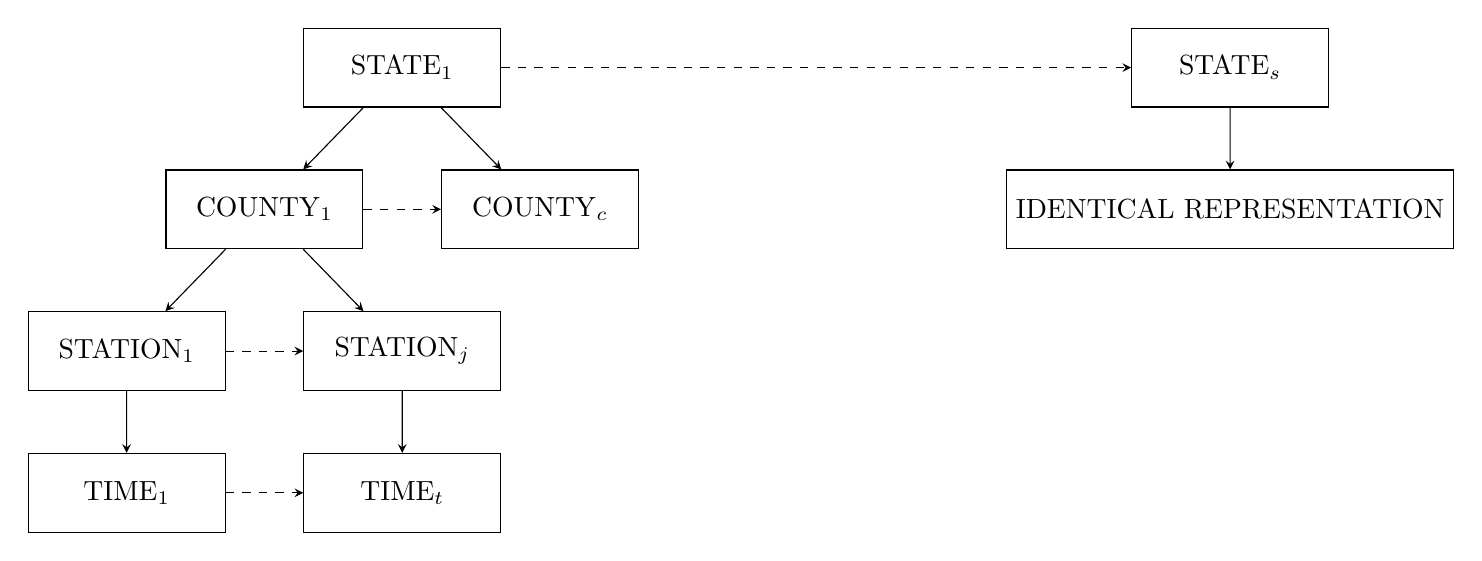
\begin{tikzpicture}[
    every node/.style={draw, minimum width=2.5cm, minimum height=1cm, font=\sffamily},
    level distance=1.8cm,
    sibling distance=3.5cm,
    ->, >=stealth
  ]

  % Nodos
  \node (state1) {$\mathrm{STATE}_{1}$}
    child {node (county1) {$\mathrm{COUNTY}_{1}$} 
      child {node (station1) {$\mathrm{STATION}_{1}$}
        child {node (time1) {$\mathrm{TIME}_{1}$}}
      }
      child {node (stationk) {$\mathrm{STATION}_{j}$}
        child {node (timet) {$\mathrm{TIME}_{t}$}}
      }
    }
    child {node (countyc) {$\mathrm{COUNTY}_{c}$}};

  \node[right=8cm of state1] (statez) {$\mathrm{STATE}_{s}$}
    child {node (others) {$\mathrm{IDENTICAL\ REPRESENTATION}$}};

  \draw[dashed] (county1) -- (countyc);
  \draw[dashed] (station1) -- (stationk);
  \draw[dashed] (time1) -- (timet);
  \draw[dashed] (state1) -- (statez);

  \end{tikzpicture}
}
\end{center}
\end{tcolorbox}
\caption{Hierarchical structure of the multilevel model: states, counties, stations, and time.}
\label{fig:hierarchy}
\end{figure}


\begin{figure}[h]
    \centering
    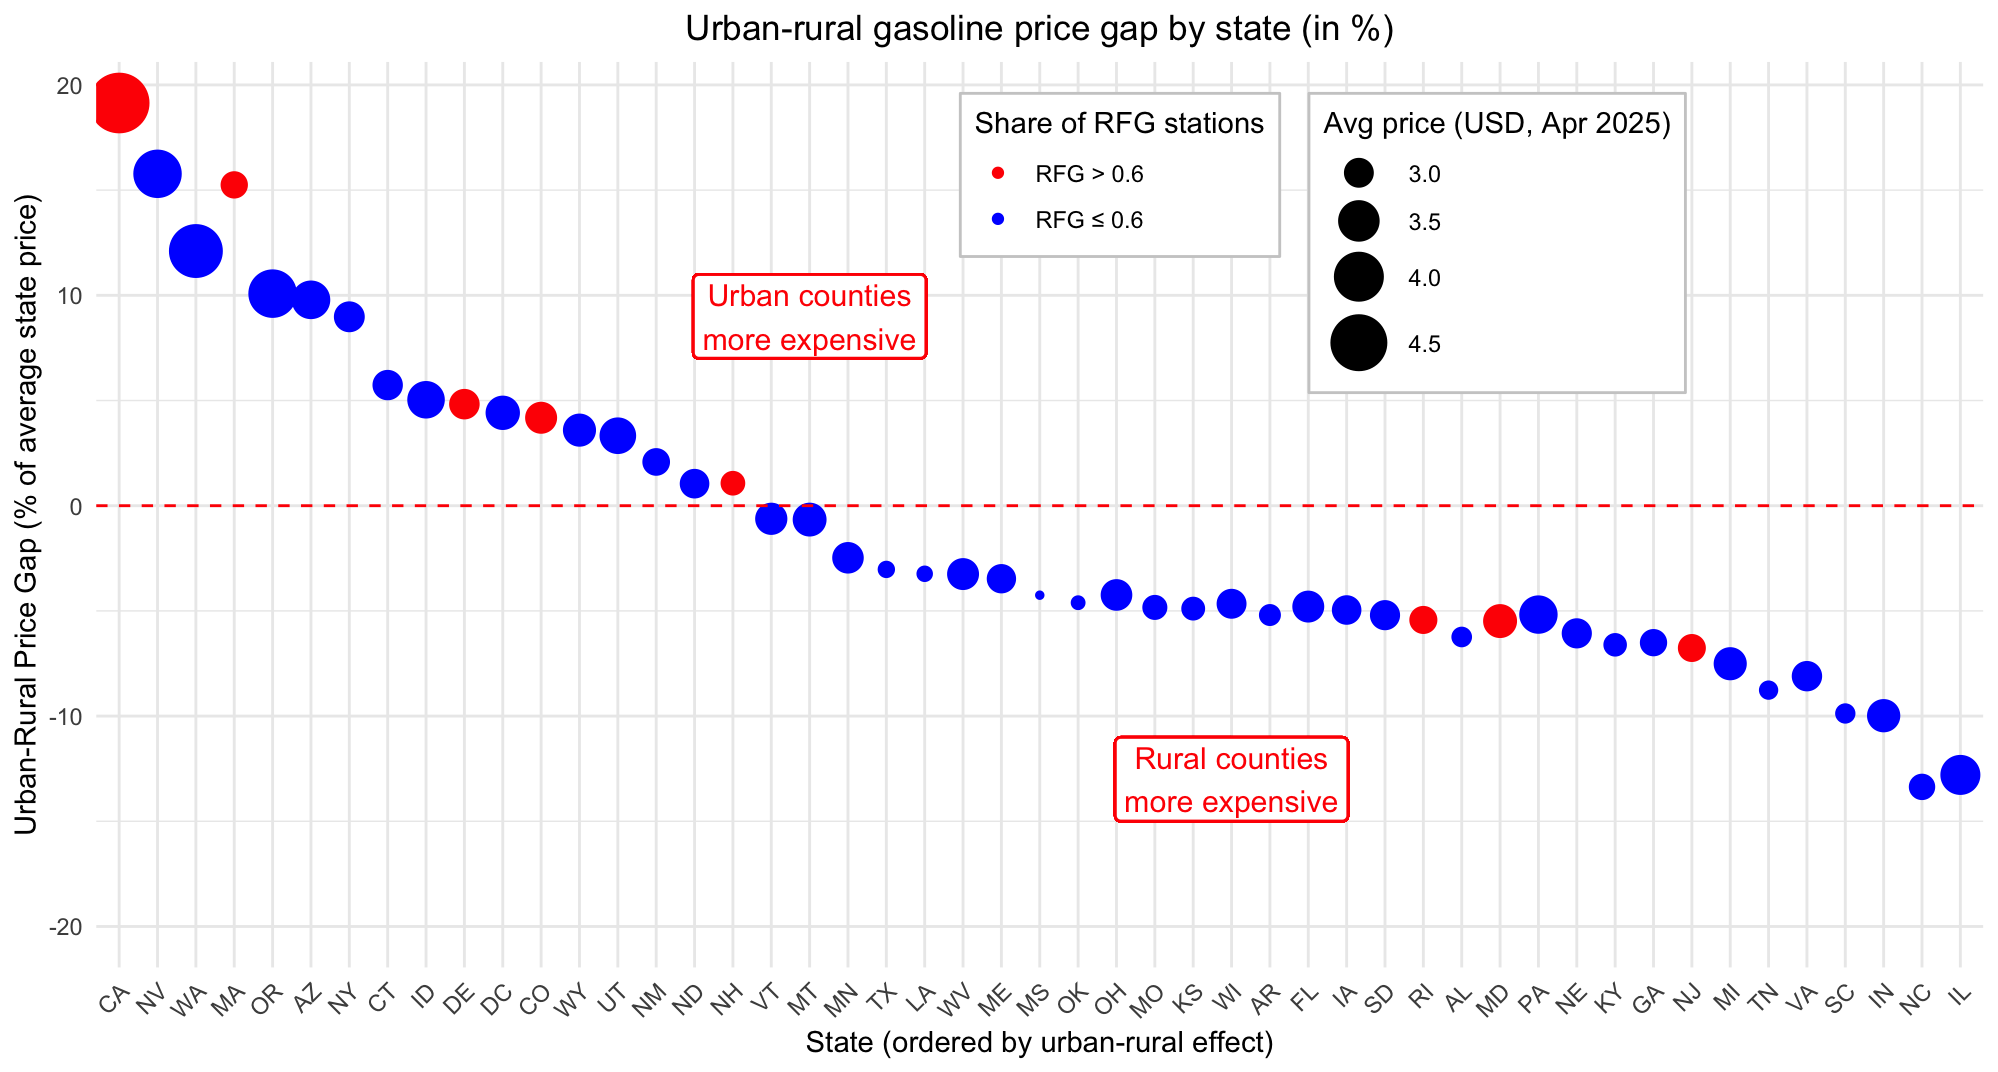
\includegraphics[width=\linewidth]{Figures/Rplot02.png}
\caption{State-Level Urban–Rural Gasoline Price Gaps (as Percentage of State Average)}

    \label{fig:Figure2}
\end{figure}

\newpage

% \appendix
% \clearpage

% \section{Tables}
% 
\begin{table}[H]
\centering
\caption{Model 3}
\label{tab:Model3}
\renewcommand{\arraystretch}{1.1}
\begin{tabular}{lccc}
\hline
\hline
\textbf{Variable} & \textbf{Coef.} & \textbf{z} & \textbf{P>|z|} \\
\hline
$\mu$ & 2.195 & 20.88 & 0.000 \\
Urban                & 0.001 & 0.09  & 0.930 \\
Weighted Tax                 & 0.023 & 7.38  & 0.000 \\
Distance to Refinery  & 0.00018 & 9.21 & 0.000 \\
Distance to Terminal  & 0.00064 & 16.73 & 0.000 \\
Reformulated Fuel (RFG)      & 0.009 & 1.12  & 0.264 \\
Population          & 2.29e-08 & 4.48 & 0.000 \\
Mean Temperature             & -0.00165 & -48.24 & 0.000 \\
January   & 0.355 & 435.74 & 0.000 \\
February  & 0.346 & 570.37 & 0.000 \\
March     & 0.455 & 665.49 & 0.000 \\
April     & 0.584 & 699.88 & 0.000 \\
May       & 0.629 & 573.76 & 0.000 \\
June      & 0.491 & 373.73 & 0.000 \\
July      & 0.538 & 383.56 & 0.000 \\
August    & 0.433 & 316.97 & 0.000 \\
September & 0.248 & 204.59 & 0.000 \\
October   & 0.179 & 185.17 & 0.000 \\
November  & 0.045 & 58.83  & 0.000 \\
Year 2025 & -0.332 & -861.90 & 0.000 \\
\hline
\hline
\multicolumn{4}{c}{\textbf{Random Effects Parameters}} \\
\hline
\textbf{Group (Parameter)} & \textbf{SD Model 3} & \textbf{SD Model 0} & \textbf{Var. (\%)} \\
\hline
State (urban2 slope)        & 0.0074551 & --       & --     \\
State ($\sigma_s^2$)        & 0.0520408 & 0,0456562    & \textbf{-14\%} \\
County ($\sigma_c^2$)       & 0.006531  & 0,0072391   & \textbf{-10\%} \\
Station ID ($\sigma_j^2$)   & 0.0189879 & 0,0189889   & \textbf{0\%} \\
Residual ($\sigma_{i}^2$)   & 0.0185978 & 0,0185978   & \textbf{0\%} \\
Total variance ($\sigma_s^2+\sigma_c^2+\sigma_j^2+\sigma_{i}^2$) & 0,1036126 & 0,090482&\textbf{15\%} \\
\hline
\hline
\multicolumn{4}{c}{\textbf{Variance Attribution by Spatial Level}} \\
\hline
\textbf{Level} & \textbf{ICC} & \textbf{SE} & \textbf{Var. (\%)} \\
\hline
State                     & 0.540 & 0.051 & \textbf{57\%} \\
County\,|\,State          & 0.610 & 0.043 & \textbf{6\%} \\
Station\,|\,County\,|\,State & 0.800 & 0.021 & \textbf{18}\% \\
Month\,|\, Station\,|\,County\,|\,State & NA & NA  & \textbf{18\%} \\
\hline
\hline
\end{tabular}

\vspace{1em}
\raggedright
\scriptsize
\textit{Note: The ICC is reported in its cumulative form, reflecting the proportion of total variance attributable to each level up to that point in the hierarchy.}
\end{table}

% \label{table}

% \clearpage
% \section{Figures}
% \begin{figure}[H]
\centering
\begin{tcolorbox}[colback=white, colframe=black, boxrule=0.4pt, arc=2pt, left=2mm, right=2mm, top=1mm, bottom=1mm]
\begin{center}
\resizebox{0.8\textwidth}{!}{
  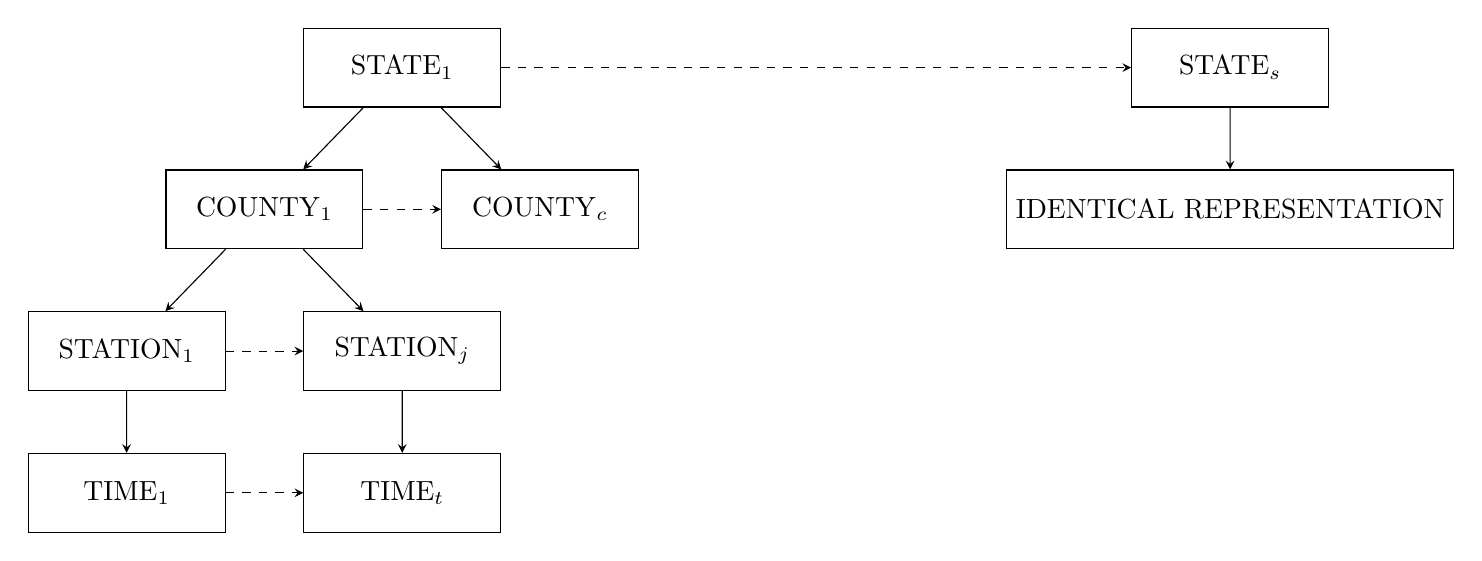
\begin{tikzpicture}[
    every node/.style={draw, minimum width=2.5cm, minimum height=1cm, font=\sffamily},
    level distance=1.8cm,
    sibling distance=3.5cm,
    ->, >=stealth
  ]

  % Nodos
  \node (state1) {$\mathrm{STATE}_{1}$}
    child {node (county1) {$\mathrm{COUNTY}_{1}$} 
      child {node (station1) {$\mathrm{STATION}_{1}$}
        child {node (time1) {$\mathrm{TIME}_{1}$}}
      }
      child {node (stationk) {$\mathrm{STATION}_{j}$}
        child {node (timet) {$\mathrm{TIME}_{t}$}}
      }
    }
    child {node (countyc) {$\mathrm{COUNTY}_{c}$}};

  \node[right=8cm of state1] (statez) {$\mathrm{STATE}_{s}$}
    child {node (others) {$\mathrm{IDENTICAL\ REPRESENTATION}$}};

  \draw[dashed] (county1) -- (countyc);
  \draw[dashed] (station1) -- (stationk);
  \draw[dashed] (time1) -- (timet);
  \draw[dashed] (state1) -- (statez);

  \end{tikzpicture}
}
\end{center}
\end{tcolorbox}
\caption{Hierarchical structure of the multilevel model: states, counties, stations, and time.}
\label{fig:hierarchy}
\end{figure}


\begin{figure}[h]
    \centering
    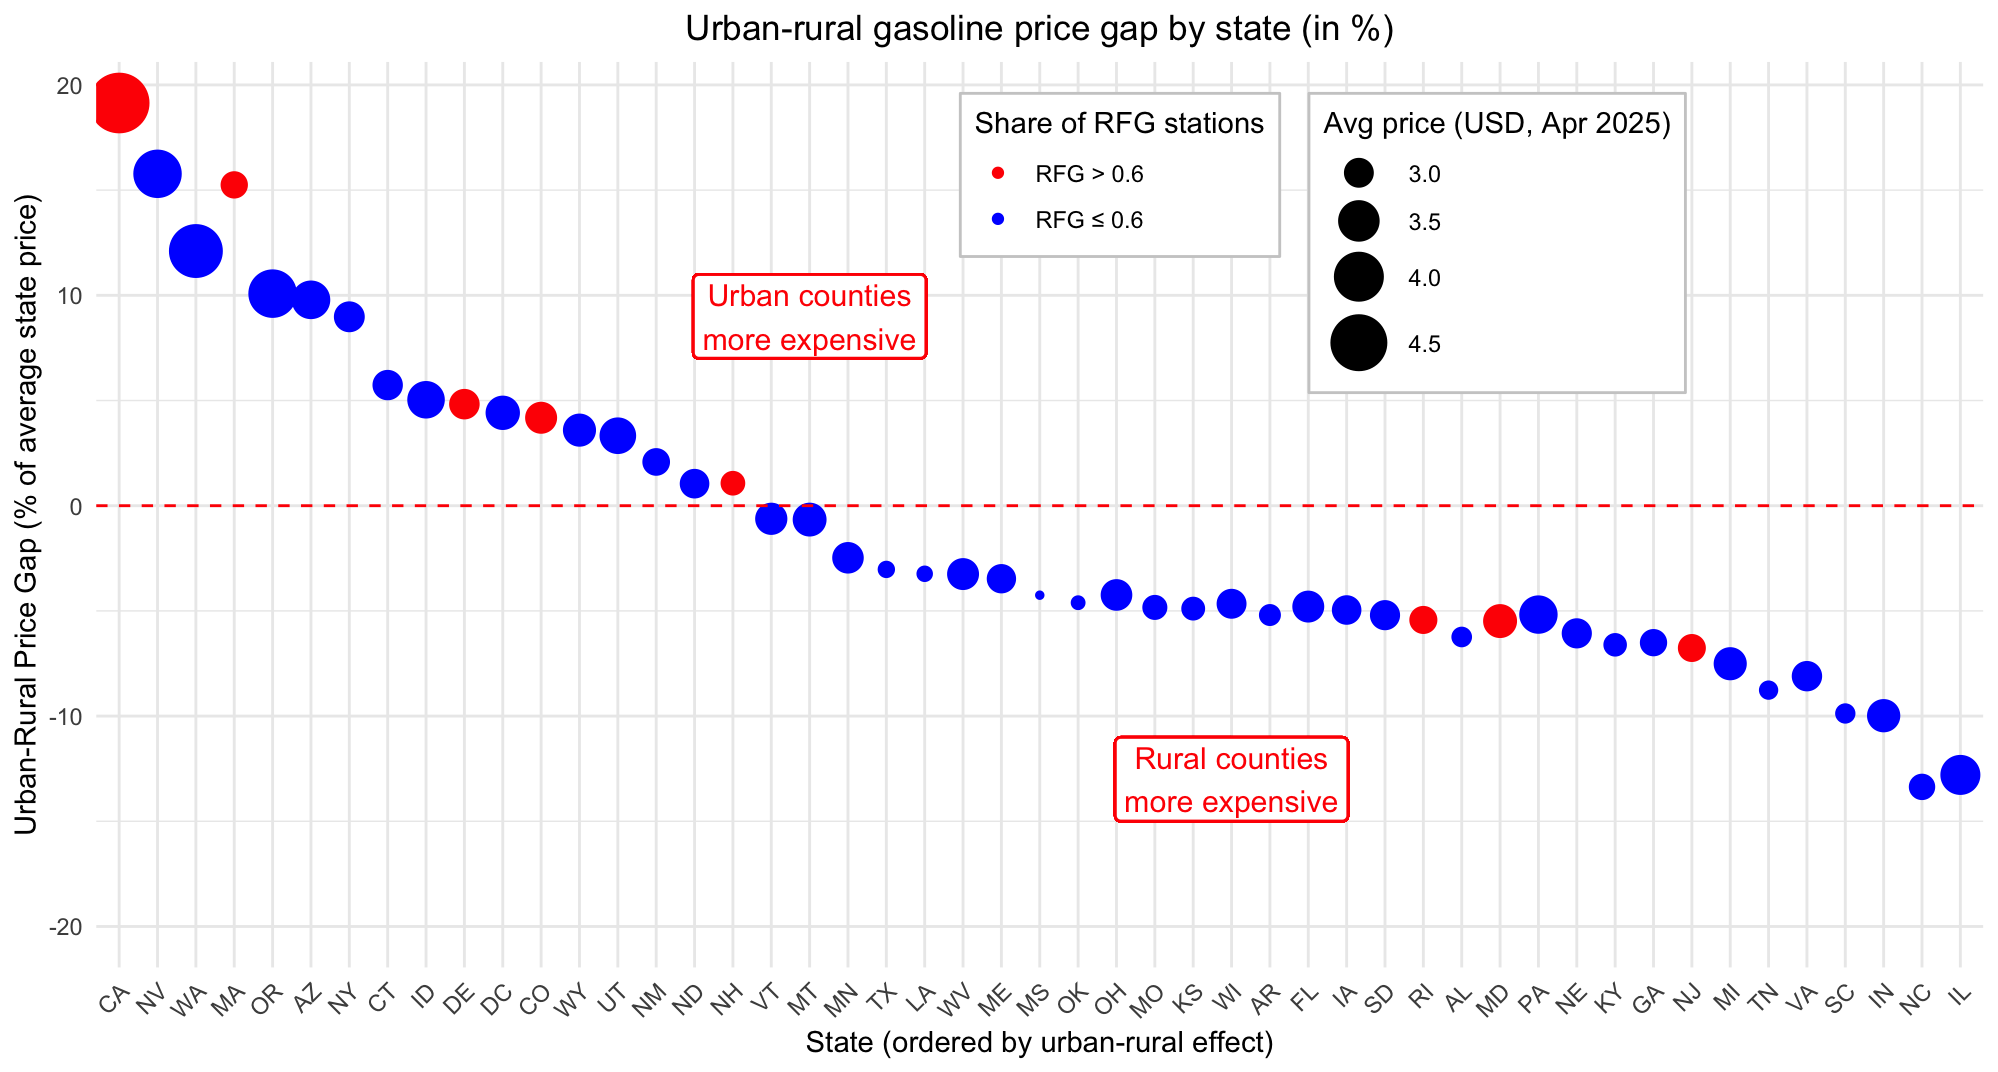
\includegraphics[width=\linewidth]{Figures/Rplot02.png}
\caption{State-Level Urban–Rural Gasoline Price Gaps (as Percentage of State Average)}

    \label{fig:Figure2}
\end{figure}

\newpage
% \label{figure}


\newpage

\bibliographystyle{apalike}
\bibliography{Bibliography}


\end{document}